%%%%%%%%%%%%%%%%%%%%%%%%%%%%%%%%%%%%%%%%%
% Beamer Presentation
% LaTeX Template
% Version 2.0 (March 8, 2022)
%
% This template originates from:
% https://www.LaTeXTemplates.com
%
% Author:
% Vel (vel@latextemplates.com)
%
% License:
% CC BY-NC-SA 4.0 (https://creativecommons.org/licenses/by-nc-sa/4.0/)
%
%%%%%%%%%%%%%%%%%%%%%%%%%%%%%%%%%%%%%%%%%

%----------------------------------------------------------------------------------------
%	PACKAGES AND OTHER DOCUMENT CONFIGURATIONS
%----------------------------------------------------------------------------------------

\documentclass[
	11pt, % Set the default font size, options include: 8pt, 9pt, 10pt, 11pt, 12pt, 14pt, 17pt, 20pt
	%t, % Uncomment to vertically align all slide content to the top of the slide, rather than the default centered
	aspectratio=169, % Uncomment to set the aspect ratio to a 16:9 ratio which matches the aspect ratio of 1080p and 4K screens and projectors
]{beamer}

\graphicspath{{Images/}{./}} % Specifies where to look for included images (trailing slash required)

\usepackage{booktabs} % Allows the use of \toprule, \midrule and \bottomrule for better rules in tables

%----------------------------------------------------------------------------------------
%	SELECT LAYOUT THEME
%----------------------------------------------------------------------------------------

% Beamer comes with a number of default layout themes which change the colors and layouts of slides. Below is a list of all themes available, uncomment each in turn to see what they look like.

%\usetheme{default}
%\usetheme{AnnArbor}
%\usetheme{Antibes}
%\usetheme{Bergen}
%\usetheme{Berkeley}
%\usetheme{Berlin}
%\usetheme{Boadilla}
%\usetheme{CambridgeUS}
%\usetheme{Copenhagen}
%\usetheme{Darmstadt}
%\usetheme{Dresden}
%\usetheme{Frankfurt}
%\usetheme{Goettingen}
%\usetheme{Hannover}
%\usetheme{Ilmenau}
%\usetheme{JuanLesPins}
%\usetheme{Luebeck}
\usetheme{Madrid}
%\usetheme{Malmoe}
%\usetheme{Marburg}
%\usetheme{Montpellier}
%\usetheme{PaloAlto}
%\usetheme{Pittsburgh}
%\usetheme{Rochester}
%\usetheme{Singapore}
%\usetheme{Szeged}
%\usetheme{Warsaw}

%----------------------------------------------------------------------------------------
%	SELECT COLOR THEME
%----------------------------------------------------------------------------------------

% Beamer comes with a number of color themes that can be applied to any layout theme to change its colors. Uncomment each of these in turn to see how they change the colors of your selected layout theme.

%\usecolortheme{albatross}
%\usecolortheme{beaver}
%\usecolortheme{beetle}
%\usecolortheme{crane}
%\usecolortheme{dolphin}
%\usecolortheme{dove}
%\usecolortheme{fly}
%\usecolortheme{lily}
%\usecolortheme{monarca}
%\usecolortheme{seagull}
%\usecolortheme{seahorse}
%\usecolortheme{spruce}
%\usecolortheme{whale}
%\usecolortheme{wolverine}

%----------------------------------------------------------------------------------------
%	SELECT FONT THEME & FONTS
%----------------------------------------------------------------------------------------

% Beamer comes with several font themes to easily change the fonts used in various parts of the presentation. Review the comments beside each one to decide if you would like to use it. Note that additional options can be specified for several of these font themes, consult the beamer documentation for more information.

\usefonttheme{default} % Typeset using the default sans serif font
%\usefonttheme{serif} % Typeset using the default serif font (make sure a sans font isn't being set as the default font if you use this option!)
%\usefonttheme{structurebold} % Typeset important structure text (titles, headlines, footlines, sidebar, etc) in bold
%\usefonttheme{structureitalicserif} % Typeset important structure text (titles, headlines, footlines, sidebar, etc) in italic serif
%\usefonttheme{structuresmallcapsserif} % Typeset important structure text (titles, headlines, footlines, sidebar, etc) in small caps serif

%------------------------------------------------

%\usepackage{mathptmx} % Use the Times font for serif text
\usepackage{palatino} % Use the Palatino font for serif text

%\usepackage{helvet} % Use the Helvetica font for sans serif text
\usepackage[default]{opensans} % Use the Open Sans font for sans serif text
%\usepackage[default]{FiraSans} % Use the Fira Sans font for sans serif text
%\usepackage[default]{lato} % Use the Lato font for sans serif text
\usepackage{filecontents} % used for reference
\usepackage[style=numeric, sorting=none, backend=biber]{biblatex} % used for reference

%----------------------------------------------------------------------------------------
%	REFERENCE
%----------------------------------------------------------------------------------------

\addbibresource{myreference.bib}

%----------------------------------------------------------------------------------------
%	SELECT INNER THEME
%----------------------------------------------------------------------------------------

% Inner themes change the styling of internal slide elements, for example: bullet points, blocks, bibliography entries, title pages, theorems, etc. Uncomment each theme in turn to see what changes it makes to your presentation.

%\useinnertheme{default}
\useinnertheme{circles}
%\useinnertheme{rectangles}
%\useinnertheme{rounded}
%\useinnertheme{inmargin}

%----------------------------------------------------------------------------------------
%	SELECT OUTER THEME
%----------------------------------------------------------------------------------------

% Outer themes change the overall layout of slides, such as: header and footer lines, sidebars and slide titles. Uncomment each theme in turn to see what changes it makes to your presentation.

%\useoutertheme{default}
%\useoutertheme{infolines}
%\useoutertheme{miniframes}
%\useoutertheme{smoothbars}
%\useoutertheme{sidebar}
%\useoutertheme{split}
%\useoutertheme{shadow}
%\useoutertheme{tree}
%\useoutertheme{smoothtree}

%\setbeamertemplate{footline} % Uncomment this line to remove the footer line in all slides
%\setbeamertemplate{footline}[page number] % Uncomment this line to replace the footer line in all slides with a simple slide count

\setbeamertemplate{navigation symbols}{} % Uncomment this line to remove the navigation symbols from the bottom of all slides
\setbeamertemplate{caption}[numbered] % numbering the figure in preentation

%----------------------------------------------------------------------------------------
%	PRESENTATION INFORMATION
%----------------------------------------------------------------------------------------

\title[Meeting 8/15]{Supervised Learning \\ Meeting 8/15} % The short title in the optional parameter appears at the bottom of every slide, the full title in the main parameter is only on the title page

% \subtitle{Optional Subtitle} % Presentation subtitle, remove this command if a subtitle isn't required

\author[Bo Han, Chen]{Bo Han, Chen} % Presenter name(s), the optional parameter can contain a shortened version to appear on the bottom of every slide, while the main parameter will appear on the title slide

\institute[NYCU]{National Yang Ming Chiao Tung University, Taiwan \\ \smallskip \textit{bhchen312551074.cs12@nycu.edu.tw}} % Your institution, the optional parameter can be used for the institution shorthand and will appear on the bottom of every slide after author names, while the required parameter is used on the title slide and can include your email address or additional information on separate lines

\date[August 15, 2023]{August 15, 2023} % Presentation date or conference/meeting name, the optional parameter can contain a shortened version to appear on the bottom of every slide, while the required parameter value is output to the title slide

%----------------------------------------------------------------------------------------

\begin{document}

%----------------------------------------------------------------------------------------
%	TITLE SLIDE
%----------------------------------------------------------------------------------------

\begin{frame}
	\titlepage % Output the title slide, automatically created using the text entered in the PRESENTATION INFORMATION block above
\end{frame}

%----------------------------------------------------------------------------------------
%	TABLE OF CONTENTS SLIDE
%----------------------------------------------------------------------------------------

% The table of contents outputs the sections and subsections that appear in your presentation, specified with the standard \section and \subsection commands. You may either display all sections and subsections on one slide with \tableofcontents, or display each section at a time on subsequent slides with \tableofcontents[pausesections]. The latter is useful if you want to step through each section and mention what you will discuss.

\begin{frame}
	\frametitle{Presentation Overview} % Slide title, remove this command for no title
	
	\tableofcontents % Output the table of contents (all sections on one slide)
	%\tableofcontents[pausesections] % Output the table of contents (break sections up across separate slides)
\end{frame}

%----------------------------------------------------------------------------------------
%	PRESENTATION BODY SLIDES
%----------------------------------------------------------------------------------------

\section{Environment}

\begin{frame}
	\frametitle{Environment}
	
	\begin{itemize}
		\item Python 3.10.12
		\begin{itemize}
			\item PyTorch 2.0.1
			\item Scikit-learn 1.2.2
		\end{itemize}
		\item platform: Google Colab
		\begin{itemize}
			\item GPU: Nvidia Tesla T4
		\end{itemize}
	\end{itemize}
\end{frame}

\section{Public Dataset}
\subsection{Oxford 102 Flower}

\begin{frame}
	\frametitle{Public Dataset}
	\framesubtitle{Oxford 102 Flower}

	\begin{itemize}
		\item preprocessing
		\begin{itemize}
			\item split the train, valid, test data (1020, 1020, 6149)
			\item resize the image data (224*224)
			\item normalization
		\end{itemize}
		\item hyperparameters
		\begin{itemize}
			\item batch size: 100
			\item epochs: 50
		\end{itemize}
		\item classifier
		\begin{itemize}
			\item VGG 19
			\item ResNet
			\begin{itemize}
				\item residual-block
			\end{itemize}
		\end{itemize}
	\end{itemize}
\end{frame}

\begin{frame}
	\frametitle{Oxford 102 Flower}
	\framesubtitle{Result}

	\begin{figure}[htbp]
		\begin{minipage}[t]{0.48\textwidth}
			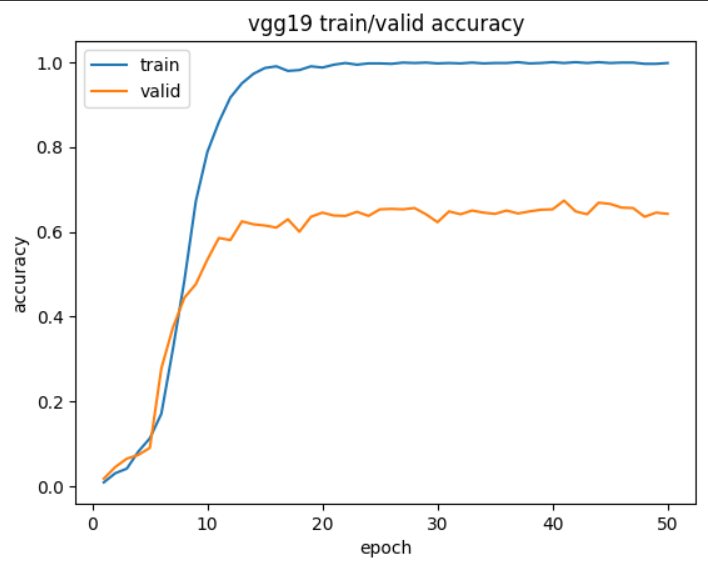
\includegraphics[width=1.0\linewidth]{vgg_accuracy.png}
			\caption{VGG training progress-accuracy}
		\end{minipage}
		\begin{minipage}[t]{0.48\textwidth}
			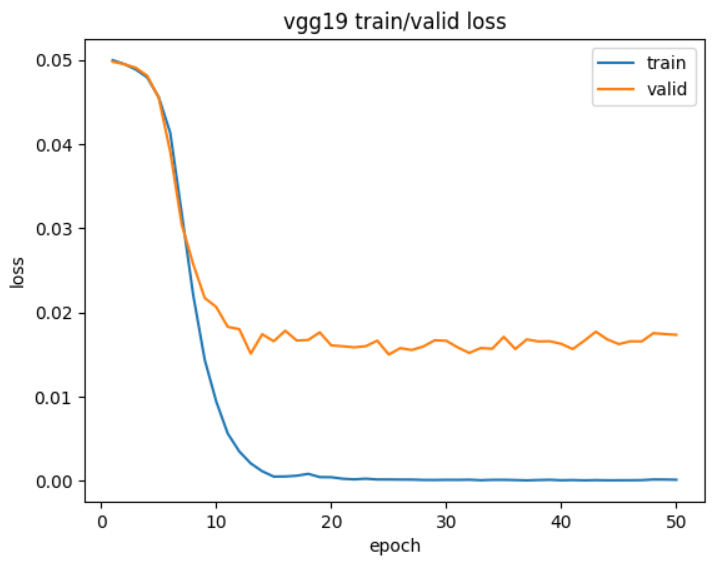
\includegraphics[width=1.0\linewidth]{vgg_loss.png}
			\caption{VGG training progress-loss}
		\end{minipage}
	\end{figure}

\end{frame}

\begin{frame}
	\frametitle{Oxford 102 Flower}
	\framesubtitle{Result}

	\begin{figure}[htbp]
		\begin{minipage}[t]{0.48\textwidth}
			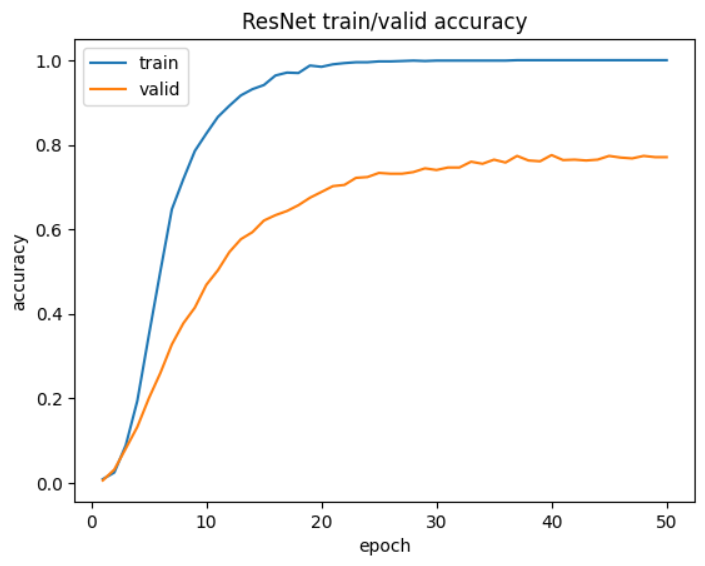
\includegraphics[width=1.0\linewidth]{resnet_accuracy.png}
			\caption{ResNet training progress-accuracy}
		\end{minipage}
		\begin{minipage}[t]{0.48\textwidth}
			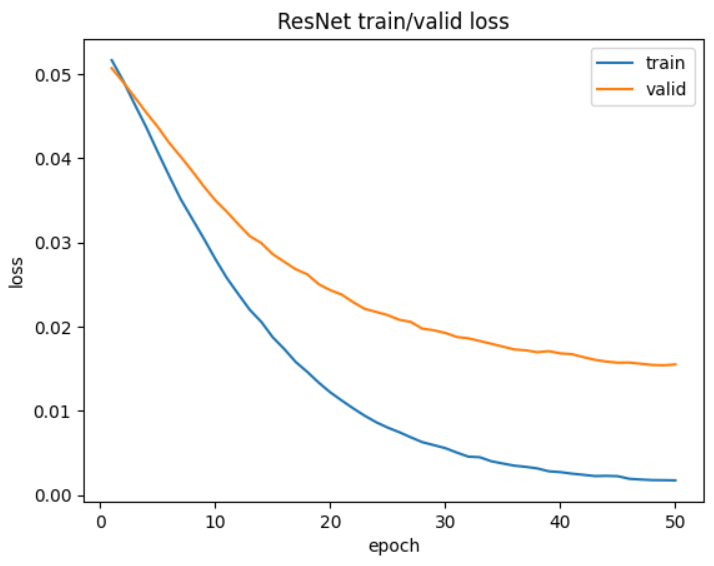
\includegraphics[width=1.0\linewidth]{resnet_loss.png}
			\caption{ResNet training progress-loss}
		\end{minipage}
	\end{figure}

\end{frame}

\begin{frame}
	\frametitle{Oxford 102 Flower}
	\framesubtitle{Result}

	\begin{center}
		\begin{tabular}{|rr|} 
			\hline
			Model&Accuracy\\          
			\hline                
			myVGG & $59.55\%$\\
			myResNet & $75.34\%$\\
			ResNet50 \cite{chen2021vision} & $90.00\%$\\
			EffNet-L2 \cite{foret2020sharpness}& $99.65\%$\\
			\hline
		\end{tabular}
	\end{center}
\end{frame}

\subsection{NSL-KDD}

\begin{frame}
	\frametitle{Public Dataset}
	\framesubtitle{NSL-KDD}

	\begin{itemize}
		\item preprocessing
		\begin{itemize}
			\item one-hot encoding
			\item min-max normalization
			\item mapping the attack class
				\begin{itemize}
					\item normal
					\item Dos
					\item Probe
					\item R2L
					\item U2R
				\end{itemize}
			\item data split (125973, 22544)
		\end{itemize}
		\item classifier
		\begin{itemize}
			\item KNN
			\item SVM
		\end{itemize}
	\end{itemize}
\end{frame}

\begin{frame}
	\frametitle{NSL-KDD}
	\framesubtitle{Result}

	\begin{figure}
		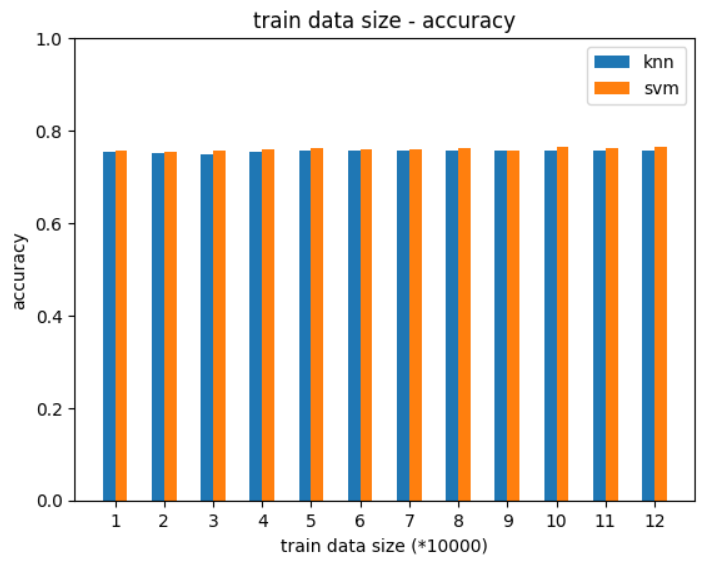
\includegraphics[width=0.5\linewidth]{nsl_kdd_train_size.png}
		\caption{train data size-accuracy on NSL-KDD}
	\end{figure}
\end{frame}

\begin{frame}
	\frametitle{NSL-KDD}
	\framesubtitle{Result}

	\begin{figure}[htbp]
		\begin{minipage}[t]{0.48\textwidth}
			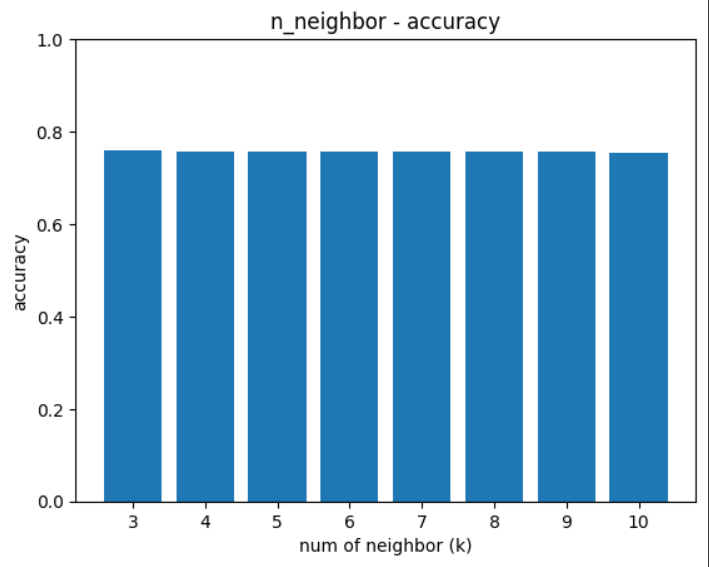
\includegraphics[width=1.0\linewidth]{knn_neighbor.png}
			\caption{KNN neighbor-accuracy}
		\end{minipage}
		\begin{minipage}[t]{0.48\textwidth}
			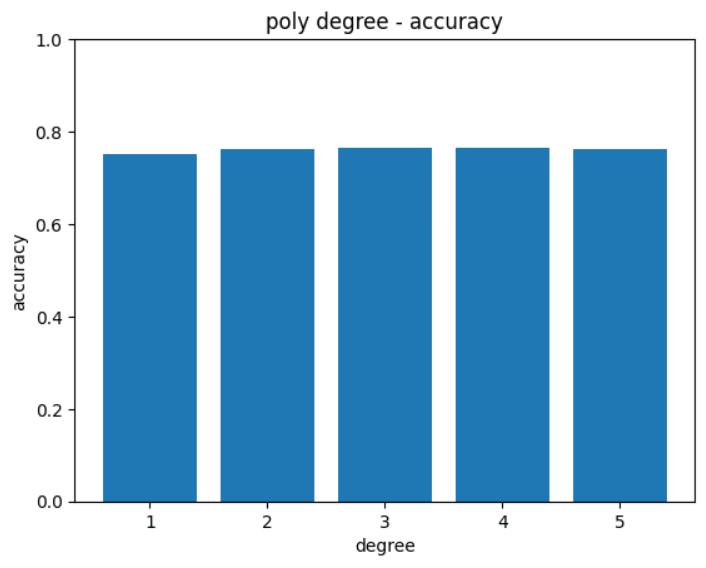
\includegraphics[width=1.0\linewidth]{svm_poly_degree.png}
			\caption{SVM degree-accuracy}
		\end{minipage}
	\end{figure}
\end{frame}

\begin{frame}
	\frametitle{NSL-KDD}
	\framesubtitle{Result}

	\begin{figure}
		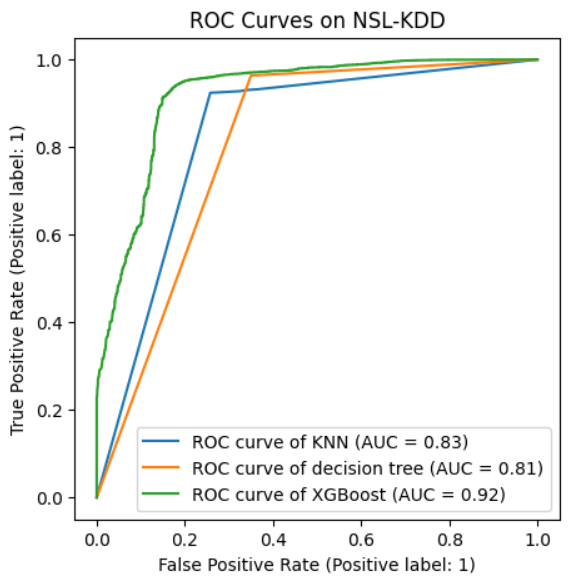
\includegraphics[width=0.35\linewidth]{roc_curve.png}
		\caption{ROC Curves on NSL-KDD}
	\end{figure}
\end{frame}

\begin{frame}
	\frametitle{NSL-KDD}
	\framesubtitle{Result}

	\begin{center}
		\begin{tabular}{|rr|} 
			\hline
			Model&Accuracy\\          
			\hline                
			myKNN & $75.71\%$\\
			mySVM & $76.44\%$\\
			ANN \cite{ingre2015performance} & $79.90\%$\\
			CNN \cite{ding2018intrusion}& $80.13\%$\\
			\hline
		\end{tabular}
	\end{center}
\end{frame}

\section{Self-Made Dataset}
\subsection{MLB}

\begin{frame}
	\frametitle{Self-Made Dataset}
	\framesubtitle{MLB}

	\begin{itemize}
		\item preprocessing
		\begin{itemize}
			\item min-max normalization
			\item reorganize the class label
		\end{itemize}
		\item classifier
		\begin{itemize}
			\item Decision Tree
			\item XGBoost
		\end{itemize}
		\item cross-validation
		\begin{itemize}
			\item Stratified K Fold with K=5
			\item 60 instances a fold
		\end{itemize}
	\end{itemize}
\end{frame}

\begin{frame}
	\frametitle{MLB}
	\framesubtitle{Result}

	\begin{figure}[htbp]
		\begin{minipage}[t]{0.48\textwidth}
			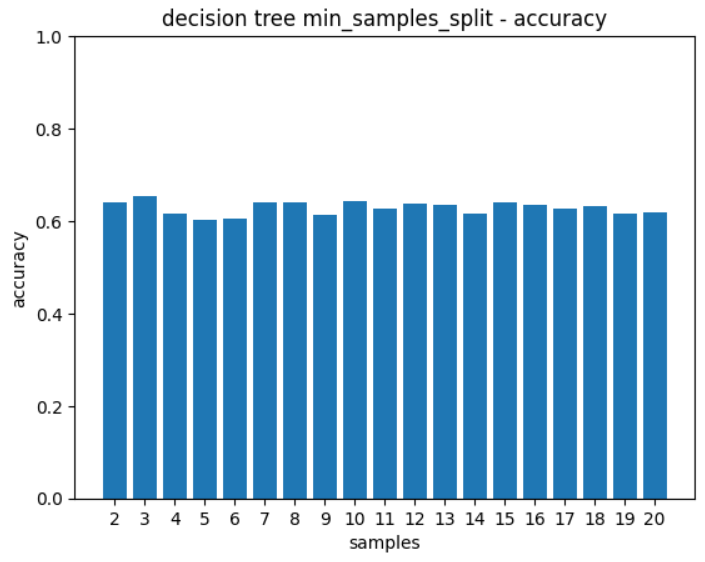
\includegraphics[width=1.0\linewidth]{decision_tree_split.png}
			\caption{Decision tree split sample-accuracy}
		\end{minipage}
		\begin{minipage}[t]{0.48\textwidth}
			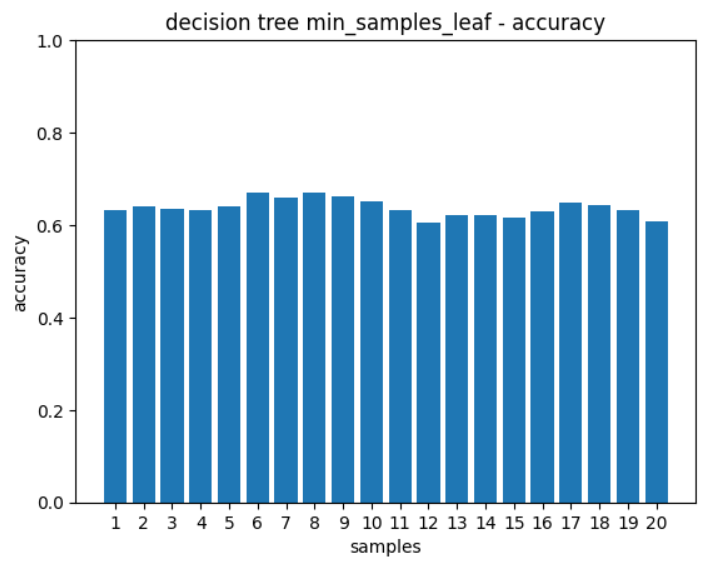
\includegraphics[width=1.0\linewidth]{decision_tree_leaf.png}
			\caption{Decision tree leaf sample-accuracy}
		\end{minipage}
	\end{figure}
\end{frame}

\begin{frame}
	\frametitle{MLB}
	\framesubtitle{Result}

	\begin{figure}[htbp]
		\begin{minipage}[t]{0.48\textwidth}
			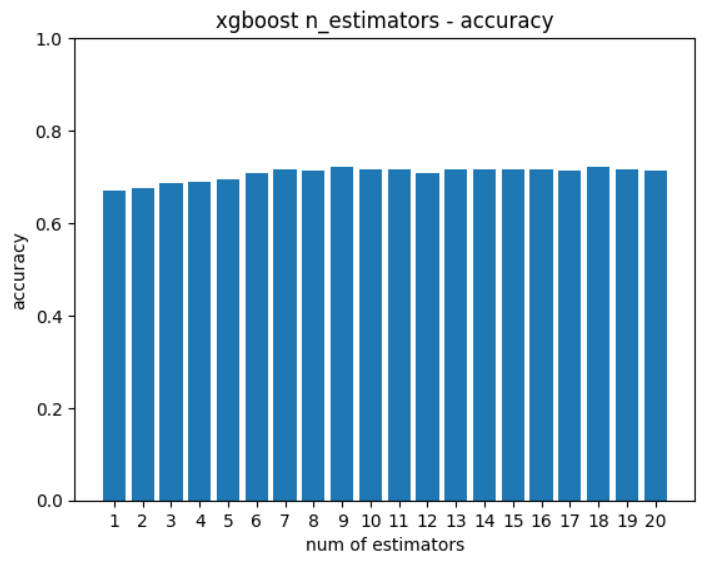
\includegraphics[width=1.0\linewidth]{xgboost_estimator.png}
			\caption{XGBoost estimator-accuracy}
		\end{minipage}
		\begin{minipage}[t]{0.48\textwidth}
			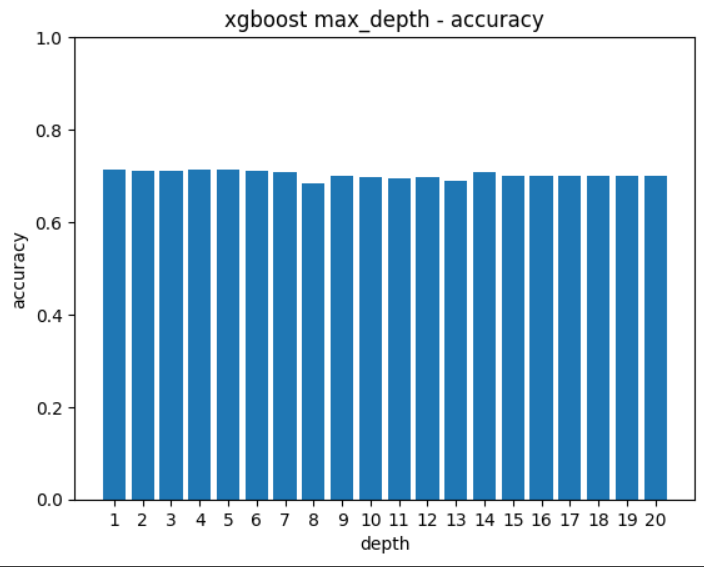
\includegraphics[width=1.0\linewidth]{xgboost_depth.png}
			\caption{XGBoost max depth-accuracy}
		\end{minipage}
	\end{figure}
\end{frame}

\section{Conclusion}

\begin{frame}
	\frametitle{Conclusion}

	\begin{itemize}
		\item more efficient way for hyperparameter tuning
		\begin{itemize}
			\item ex: evolutionary algorithm
		\end{itemize}
		\item try different preprocessing method
		\begin{itemize}
			\item ex: dimensionality reduction 
		\end{itemize}
	\end{itemize}
\end{frame}

% \begin{frame}
% 	\frametitle{Public Dataset}
	
% 	\begin{itemize}
% 		\item public image dataset
% 		\begin{itemize}
% 			\item Oxford 102 Flower
% 			\item source: Visual Gepmetry Group website
% 			\item 8189 images consist of 12 categories
% 			\item classifier: CNN based network (ResNet), XGBoost
% 		\end{itemize}
% 		\item public non-image dataset
% 		\begin{itemize}
% 			\item NSL-KDD
% 			\item source: UNB website
% 			\item 41 features for each instance, 4 classes of attack
% 			\item classifier: KNN, SVM
% 		\end{itemize}
% 	\end{itemize}
% \end{frame}

% \begin{frame}
% 	\frametitle{Self-Made Dataset}

% 	\begin{itemize}
% 		\item MLB Team Performance Prediction
% 		\begin{itemize}
% 			\item can statistics help teams win the game?
% 			\item source: Baseball Reference website
% 			\item features: the statistics of each team from 2013-2022
% 			\item three main field: batting, pitching, fielding
% 			\item classification: 50\%+ Win-Loss percentage in the regular season or not
% 			\item classifier: random forest, XGBoost
% 		\end{itemize}
% 	\end{itemize}
% \end{frame}

% \section{Motivation}

% \subsection{Issues of Deep Learning Models}

% \begin{frame}
% 	\frametitle{Motivation}
% 	\framesubtitle{Issues of Deep Learning Models}

% 	\begin{itemize}
% 		\item Spatio-temporal network prediction
% 			\begin{itemize}
% 				\item internet traffic, transportation network flow, etc
% 				\item BSS station demand prediction
% 			\end{itemize}
% 		\item Model Design
% 			\begin{itemize}
% 				\item Background knowledge is needed
% 				\item Time-consuming procedure
% 			\end{itemize}
% 		% \item Background knowledge is needed for designing a well model
% 		% \item Time-consuming procedure for building model architecture manually
% 		% \item Automatically configuring a DL model becomes a critical issue
% 	\end{itemize}

% 	\begin{block}{Objective}
% 		Automatically create a model with well-predicting performance on BSS prediction problem
% 	\end{block}
% \end{frame}

%------------------------------------------------

% \section{Method}

% \subsection{Neural Architecture Search (NAS)}

% \begin{frame}
% 	\frametitle{Method}
% 	\framesubtitle{Neural Architecture Search (NAS)}
	
% 	\begin{itemize}
% 		\item Spatio-Temporal Network Prediction
% 			\begin{itemize}
% 				% \item CNN and LSTM layer is used to capture the spatial / temporal dependency,\
% 				% the model is based on STDN \cite{yao2019revisiting}
% 				\item CNN / LSTM layer
% 				\item Based on STDN \cite{yao2019revisiting}
% 			\end{itemize}
% 	\end{itemize}

% 	\begin{itemize}
% 		\item Cell \& Linear Choice Block
% 		\begin{enumerate}
% 			\item Kernel size
% 			\item Max/avg pooling
% 			\item Activation functions choice blocks\
% 			% will be sampled equally in training and searching phase
% 		\end{enumerate}
% 	\end{itemize}

% 	\begin{itemize}
% 		\item Supernet \cite{guo2020single}
% 		\begin{itemize}
% 			\item Consist of several choice block
% 			\item Training all architectures' weights uniformly\
% 			% during training supernet
% 		\end{itemize}
% 	\end{itemize}

% \end{frame}

% \begin{frame}
% 	\frametitle{Method}
% 	\framesubtitle{NAS - Linear Choice Block}

% 	\begin{figure}
% 		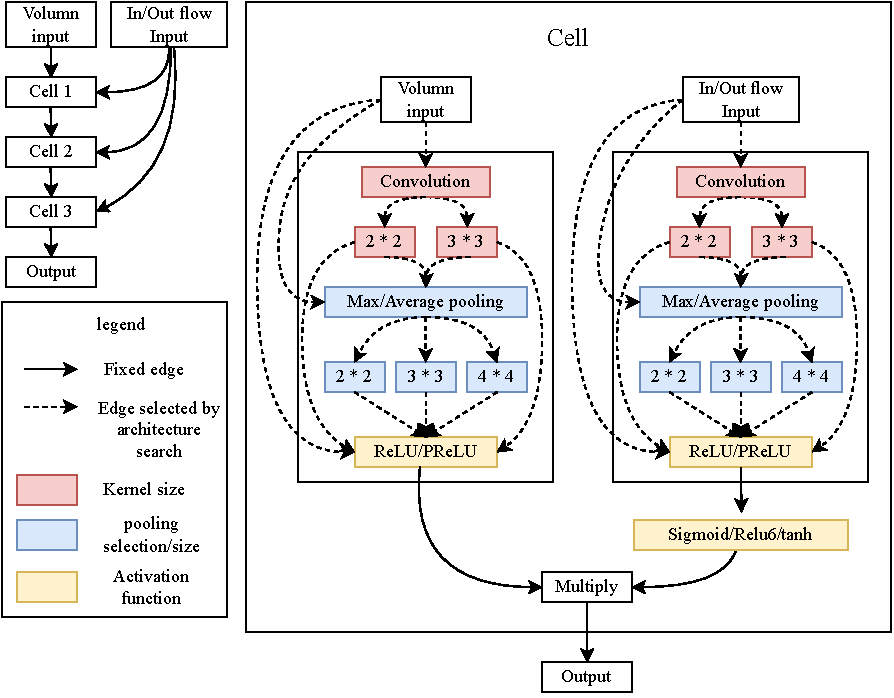
\includegraphics[width=0.5\linewidth]{cell.pdf}
% 		\caption{Cell Component}
% 	\end{figure}
% \end{frame}

% \begin{frame}
% 	\frametitle{Method}
% 	\framesubtitle{NAS - Framework Phase}

% 	% The framework is designed to operated through following phase

% 	% \begin{enumerate}
% 	% 	\item Training supernet - training all architecture in supernet, choice block will be sampled equally during this phase \cite{guo2020single}
% 	% 	\item Searching - find the best architecture by searching strategy algorithm, Adaptive Simulated Annealing Genetic Algorithm\
% 	% 	(ASAGA) is used in the framework
% 	% 	\item Retrain - train the model architecture found in searching phase
% 	% 	\item Evaluate - after training, the model will be evaluate by the test dataset
% 	% \end{enumerate}

% 	\begin{figure}
% 		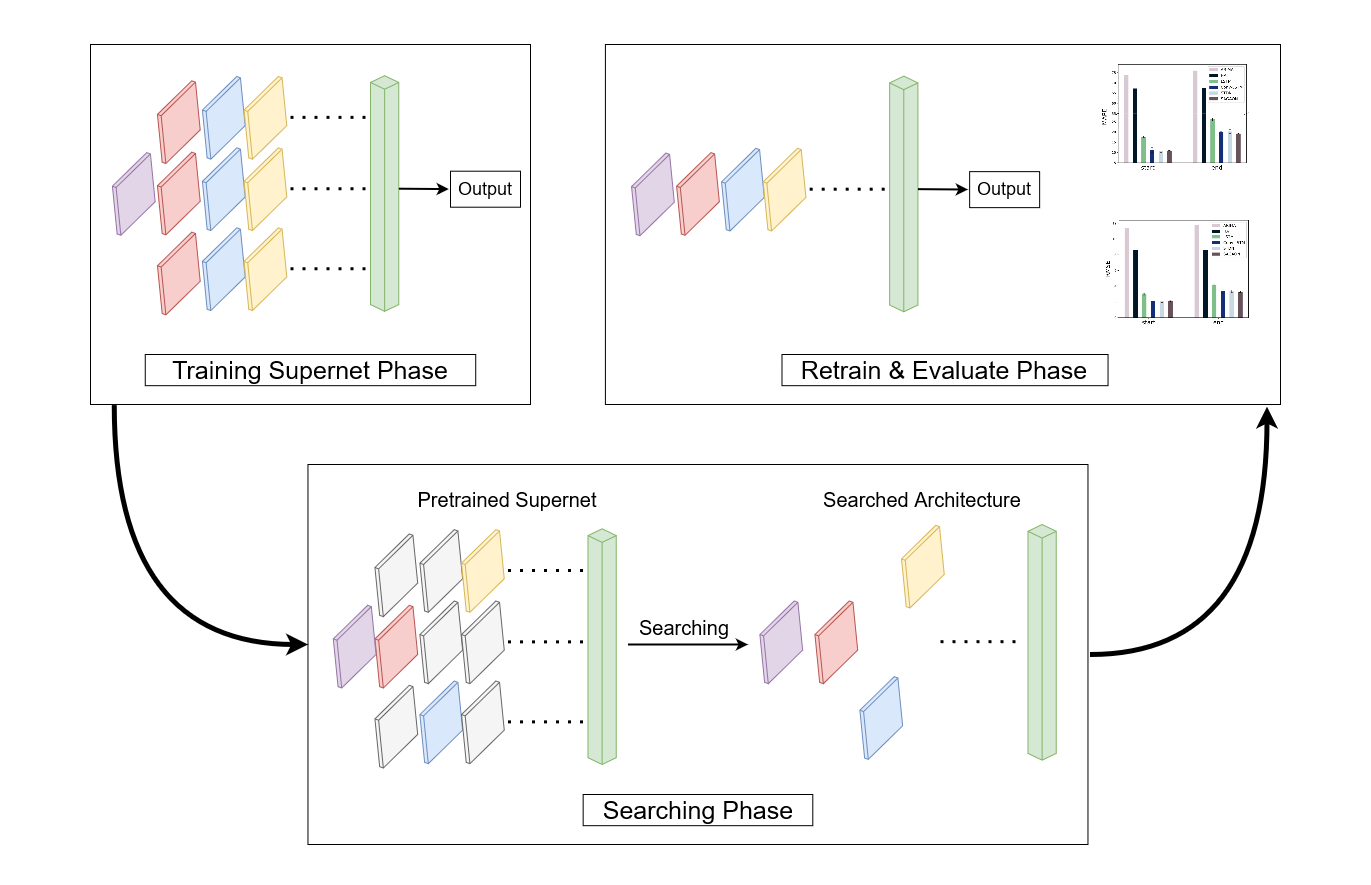
\includegraphics[width=0.61\linewidth]{phase.png}
% 		\caption{Framework Phase}
% 	\end{figure}


% \end{frame}

% \subsection{Adaptive Simulated Annealing Genetic Algorithm}

% \begin{frame}
% 	\frametitle{Method}
% 	\framesubtitle{Adaptive Simulated Annealing Genetic Algorithm (ASAGA)}

% 	\begin{itemize}
% 		% \item Based on genetic algorithm but applying SA to select the individuals of next generation \cite{mahfoud1995parallel}
% 		\item SA is applied for selection \cite{mahfoud1995parallel}
% 		\item Accepting offspring with worse RMSE result
% 		\item Sharing architecture weights
% 		% \item The weights of architectures are shared from the trained supernet
% 	\end{itemize}

% 	\begin{figure}
% 		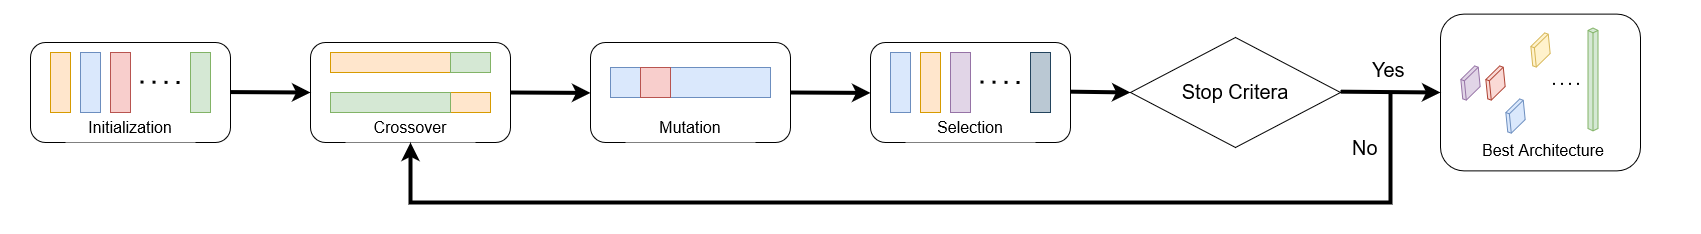
\includegraphics[width=1.0\linewidth]{ASAGA_flow.png}
% 		\caption{ASAGA Flow Chart}
% 	\end{figure}

% \end{frame}

% \begin{frame}
% 	\frametitle{Method}
% 	\framesubtitle{ASAGA - Crossover, Mutation and Selection}

% 	\begin{columns}
% 		\begin{column}{.4\textwidth}
% 			\begin{figure}
% 				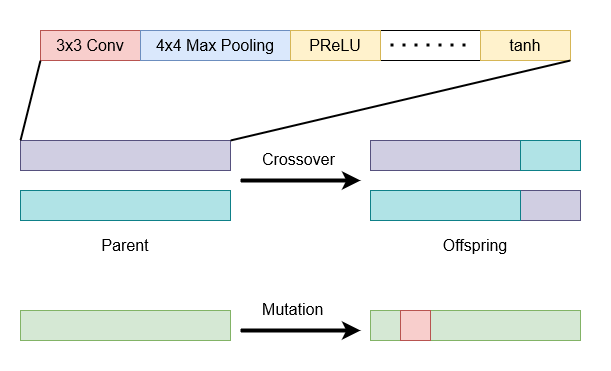
\includegraphics[width=0.9\linewidth]{ASAGA_operation.png}
% 				\caption{ASAGA Operation \& Encodeing}
% 			\end{figure}
% 		\end{column}

% 		\begin{column}{.6\textwidth}
% 			\begin{itemize}
% 				\item Architecture encoding
% 				\item Crossover and mutate on single point
% 				\item SA selection -  prevent local optimum
% 			\end{itemize}
% 		\end{column}
% 	\end{columns}

% 	\begin{block}{Efficiency of NAS Framework}
% 		Instead of training different model but training supernet and finding best model by ASAGA
% 	\end{block}

% \end{frame}

% \begin{frame}
% 	\frametitle{Method}
% 	\framesubtitle{ASAGA - Selection}

	
% \end{frame}

%------------------------------------------------

% \section{Result}

% \begin{frame}
% 	\frametitle{Result}
	
% 	\begin{figure}[htbp]
% 		\begin{minipage}[t]{0.48\textwidth}
% 			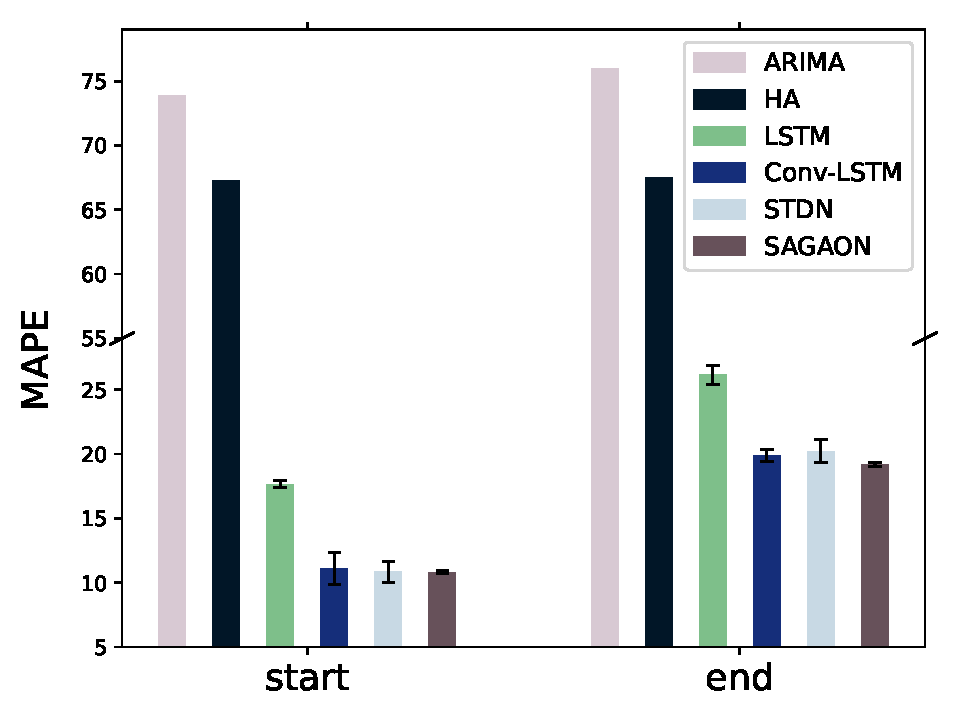
\includegraphics[width=1.0\linewidth]{station_level_MAPE.pdf}
% 			\caption{MAPE Result}
% 		\end{minipage}
% 		\begin{minipage}[t]{0.48\textwidth}
% 			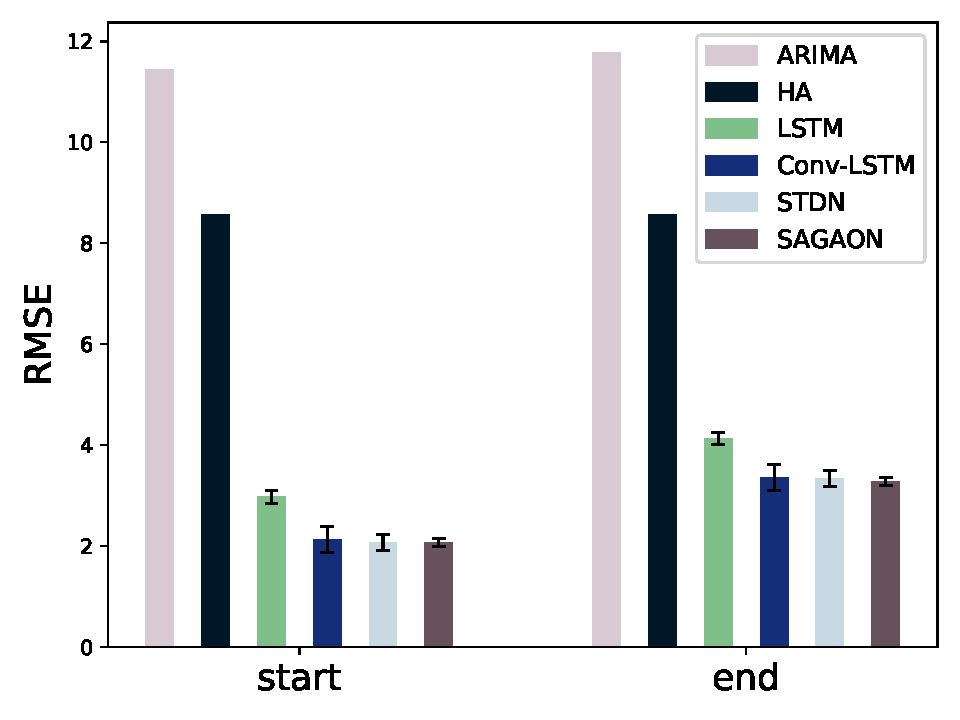
\includegraphics[width=1.0\linewidth]{station_level_RMSE.pdf}
% 			\caption{RMSE Result}
% 		\end{minipage}
% 	\end{figure}

% \end{frame}

%------------------------------------------------

% \section{Future Work}

% \begin{frame}
% 	\frametitle{Future Work}

% 	\begin{itemize}
% 		\item Expand searching space and supernet with more architecture
% 		\item Analyze factors of stations with low accuracy
% 		\item Decrease training cost to apply in real world BSS
% 	\end{itemize}
% \end{frame}

%------------------------------------------------

% \section{Acknowledgements}

% \begin{frame}
% 	\frametitle{Acknowledgements}
	
% 	\textbf{Thanks for Huge Experiment Support and \\ Quality Improvement by}
% 		\begin{itemize}
% 			\item Chao-Yen Huang
% 			\item Yun-Ye Cai
% 		\end{itemize}
% 	\vspace*{1cm}
% 	\textbf{Thanks for advising by}
% 		\begin{itemize}
% 			\item Chun-Wei Tsai
% 		\end{itemize}
% \end{frame}

%------------------------------------------------

\section{References}

\begin{frame}
	\frametitle{References}

	\printbibliography
\end{frame}

%----------------------------------------------------------------------------------------
%	CLOSING SLIDE
%----------------------------------------------------------------------------------------

\section{Q \& A}

\begin{frame}
    \frametitle{Q \& A}
	\begin{center}
		{\Huge Thanks for Listening}
		
		\bigskip\bigskip % Vertical whitespace
		
		{\LARGE Q \& A}

		% \bigskip\bigskip
		% Contact Me: b083040012@g-mail.nsysu.edu.tw
	\end{center}
\end{frame}

%----------------------------------------------------------------------------------------

\end{document} 